\documentclass{article}
\usepackage[a4paper, margin=1in]{geometry}
\usepackage{graphicx}
\usepackage{array}
\usepackage{booktabs}
\usepackage{hyperref}

\title{COP290: C Lab | Spreadsheet Program}
\author{Dheeraj HJ - 2022EE11704}

\date{}
\begin{document}

\maketitle

\section{Introduction}
This document provides an overview of the spreadsheet program written in C. It explains the design structure of the program along with the challenges faced during its development.

\section{Program Structure}
Below is a diagram showing key files and data structures:

\begin{figure}[h]
    \centering
    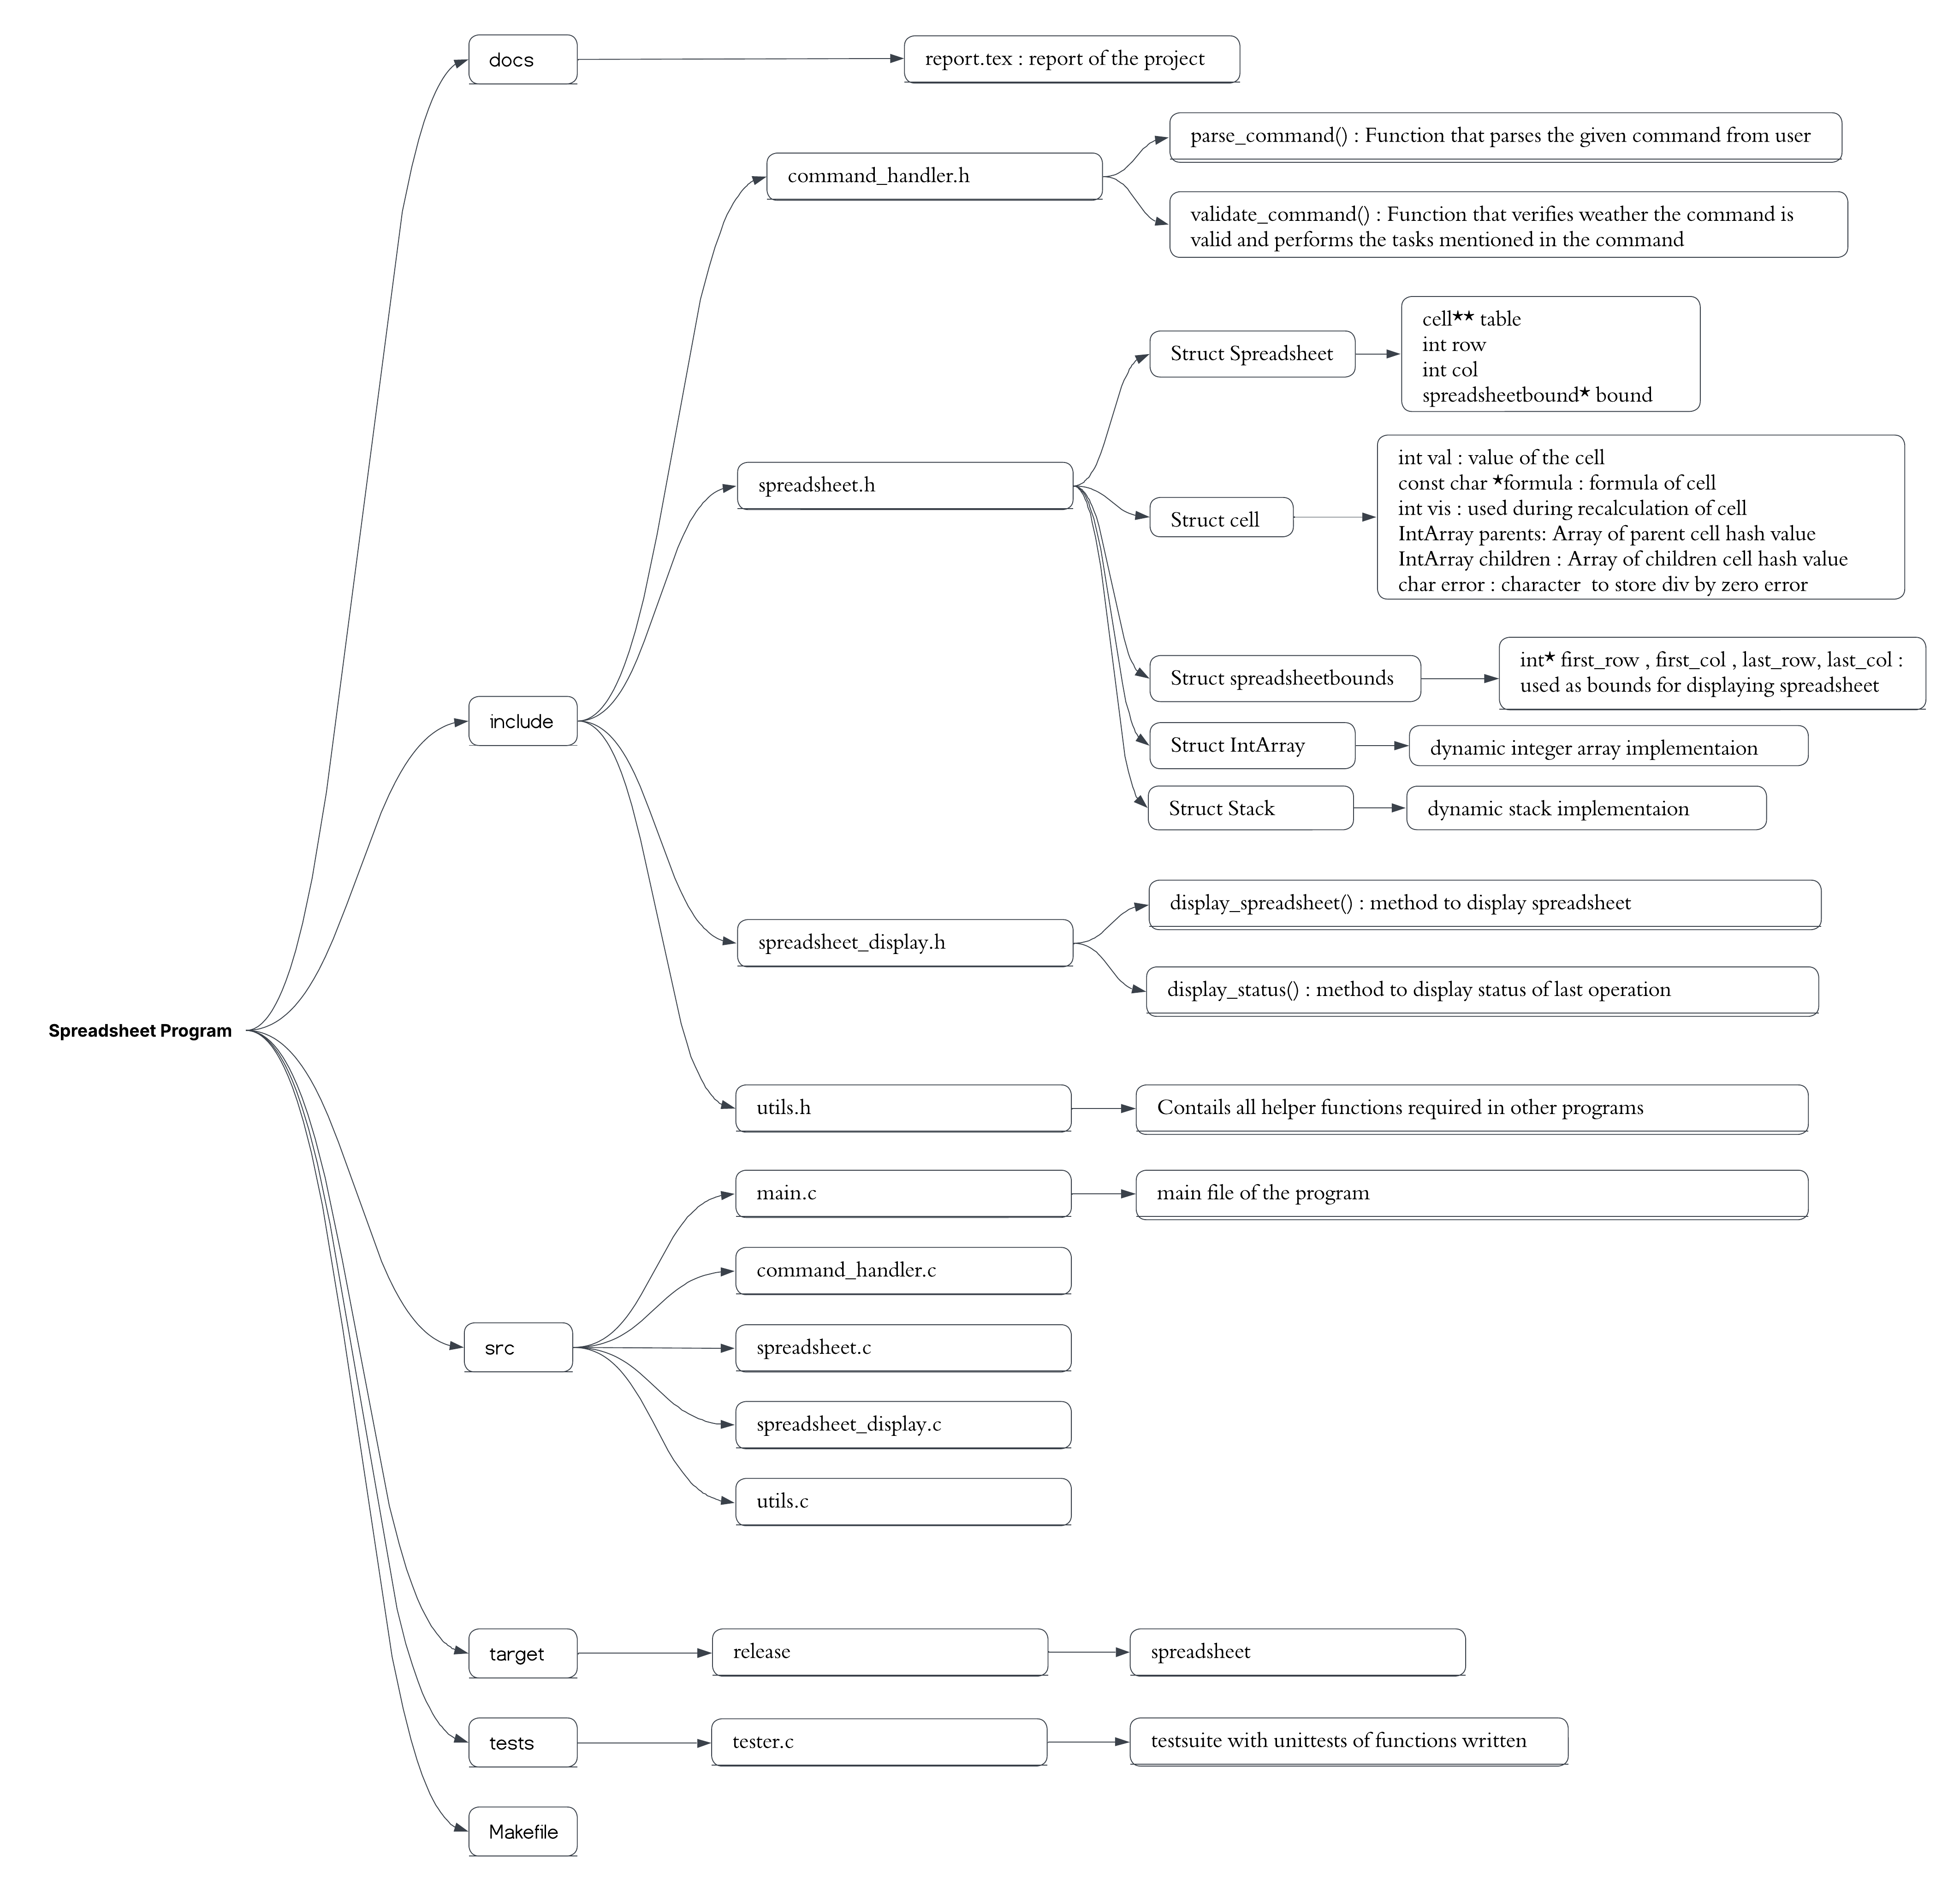
\includegraphics[width=1\textwidth]{mind-map.png}
    \caption{Program Structure}
\end{figure}

\section{Design}
The program is designed using a modular approach with the following key components:
\begin{itemize}
    \item \textbf{Command Handler:} This module is responsible for parsing and executing commands. It categorizes different commands and ensures their validity.
    \item \textbf{Spreadsheet Core:} This module manages all the data structures used in the program. It handles cell data and computations.
    \item \textbf{Display Module:} This module is responsible for rendering the spreadsheet interface, ensuring proper formatting for the user.
    \item \textbf{Utility Functions:} A set of helper functions used for various tasks throughout the program.
    \item For re-computation of cells, a directed graph-like data structure is used. Each cell maintains details of its parent and child cells using an integer hash value.
    \item To ensure proper re-computation, topological sorting is used to determine the correct order in which cells need to be updated.
    \item Dynamic resizing of integer arrays and stacks is implemented to optimize performance and ensure efficient memory usage.
    \item An error flag is maintained to handle division-by-zero errors during recalculation and display.
\end{itemize}

\textbf{Workflow} of the program:
\begin{itemize}
    \item When a user inputs a command, the main function forwards it to the parsing function.
    \item The command is validated and categorized into different types if it is valid.
    \item If the command involves dependencies on other cells, cycle detection is performed.
    \item Parent-child relationships between cells are established. For example, in a command like \texttt{A1 = B1 + 1}, \texttt{A1} is treated as a child of \texttt{B1}, and \texttt{B1} as a parent of \texttt{A1}. This ensures that when a cell's value changes, all its dependent cells are re-computed. The parent relationship is also used to remove dependencies when a new value is assigned to a cell.
    \item The expression is stored in the cell, and its value is updated accordingly. The re-computation of dependent cells is triggered using a topological sorting algorithm.
    \item The spreadsheet and its status are displayed depending on whether the program is in output-enabled or output-disabled mode.
\end{itemize}

\section{Error Handling}
The program reports the following errors or edge cases when encountered:
\begin{itemize}
    \item \textbf{Command not recognized:} If the input does not match any known command.
    \item \textbf{INVALID reference to cell:} If a referenced cell in an expression is out of bounds or incorrectly formatted (e.g., \texttt{A88A} or \texttt{AAA99} in a 5×5 sheet).
    \item \textbf{INVALID expression:} If an expression is syntactically incorrect, such as \texttt{A10/+A3}, \texttt{A2--}, or \texttt{A20+A29} in a 10×10 spreadsheet.
    \item \textbf{INVALID range:} If a specified range is not valid, e.g., \texttt{MIN(D20:A1)} or \texttt{SUM(A2:A20)} in a spreadsheet smaller than the referenced range.
    \item \textbf{Self-reference:} If a cell references itself, e.g., \texttt{A1 = A1 + 2} or \texttt{A2 = AVG(A1:B4)}.
    \item \textbf{Cycle Formation:} If cell dependencies create a circular reference, e.g., \texttt{A1} $\rightarrow$ \texttt{A2} $\rightarrow$ \texttt{A3} $\rightarrow$ \texttt{A1}.
\end{itemize}

\section{Challenges Faced}
\begin{itemize}
    \item Segmentation faults occurred due to improper memory management, which took time to debug and fix.
    \item The introduction of an explicit error display mechanism (\texttt{ERR}) required modifications to the existing error-handling approach, which initially only reported errors in the status.
    \item The test suite was not built continuously throughout the development process, leading to difficulties in comprehensive testing at the end.
    \item Performance inconsistencies were observed for large computations, such as \texttt{AVG(A2:ZZZ999)}. The computation time varied from approximately 0.9–1 second on my laptop to around 0.6 seconds on a friend's laptop.
\end{itemize}

\section{Demo and Source Code}
Video Demo: \href{https://drive.google.com/drive/folders/1JQE8CMu1abhWop8P4bJsiEpsB6zOg36A?usp=sharing}{Click here}\\
GitHub Repository: \href{https://github.com/dheeraj-hj/Spreadsheet-Program-in-C}{Link}

\end{document}
